\documentclass[letterpaper,11pt]{article}
\usepackage{graphicx}
\graphicspath{ {images/} }
\usepackage{wrapfig}
\usepackage{lipsum}
\newlength{\outerbordwidth}
\pagestyle{empty}
\raggedbottom
\raggedright
\usepackage[svgnames]{xcolor}
\usepackage{framed}
\usepackage{tocloft}
\usepackage{amsmath}
\usepackage{etoolbox}
\robustify\cftdotfill

%-----------------------------------------------------------
%Edit these values as you see fit
\setlength{\outerbordwidth}{3pt}  % Width of border outside of title bars
\definecolor{shadecolor}{gray}{0.75}  % Outer background color of title bars (0 = black, 1 = white)
\definecolor{shadecolorB}{gray}{0.93}  % Inner background color of title bars

%-----------------------------------------------------------
%Margin setup
\setlength{\evensidemargin}{-0.25in}
\setlength{\headheight}{-0.25in}
\setlength{\headsep}{0in}
\setlength{\oddsidemargin}{-0.25in}
\setlength{\paperheight}{11in}
\setlength{\paperwidth}{8.5in}
\setlength{\tabcolsep}{0in}
\setlength{\textheight}{9.75in}
\setlength{\textwidth}{7in}
\setlength{\topmargin}{-0.3in}
\setlength{\topskip}{0in}
\setlength{\voffset}{0.1in}

%-----------------------------------------------------------
%Custom commands
\newcommand{\resitem}[1]{\item #1 \vspace{-2pt}}
\newcommand{\resheading}[1]{\vspace{8pt}
  \parbox{\textwidth}{\setlength{\FrameSep}{\outerbordwidth}
    \begin{shaded}

\setlength{\fboxsep}{0pt}\framebox[\textwidth][l]{\setlength{\fboxsep}{4pt}\fcolorbox{shadecolorB}{shadecolorB}{\textbf{\sffamily{\mbox{~}\makebox[6.762in][l]{\large #1} \vphantom{p\^{E}}}}}}
    \end{shaded}
  }\vspace{-5pt}
}

\newcommand{\ressubheading}[4]{
\begin{tabular*}{6.5in}{l@{\cftdotfill{\cftsecdotsep}\extracolsep{\fill}}r}
		\textbf{#1} & #2 \\
		\textit{#3} & \textit{#4} \\
\end{tabular*}\vspace{-6pt}}
%--------------------------------------------------------------------------------------
\begin{document}

%---------------------Personal Information--------------------------------
%---------------------Image Inserted---------------------------------------
\begin{wrapfigure}{r}{4.5cm}
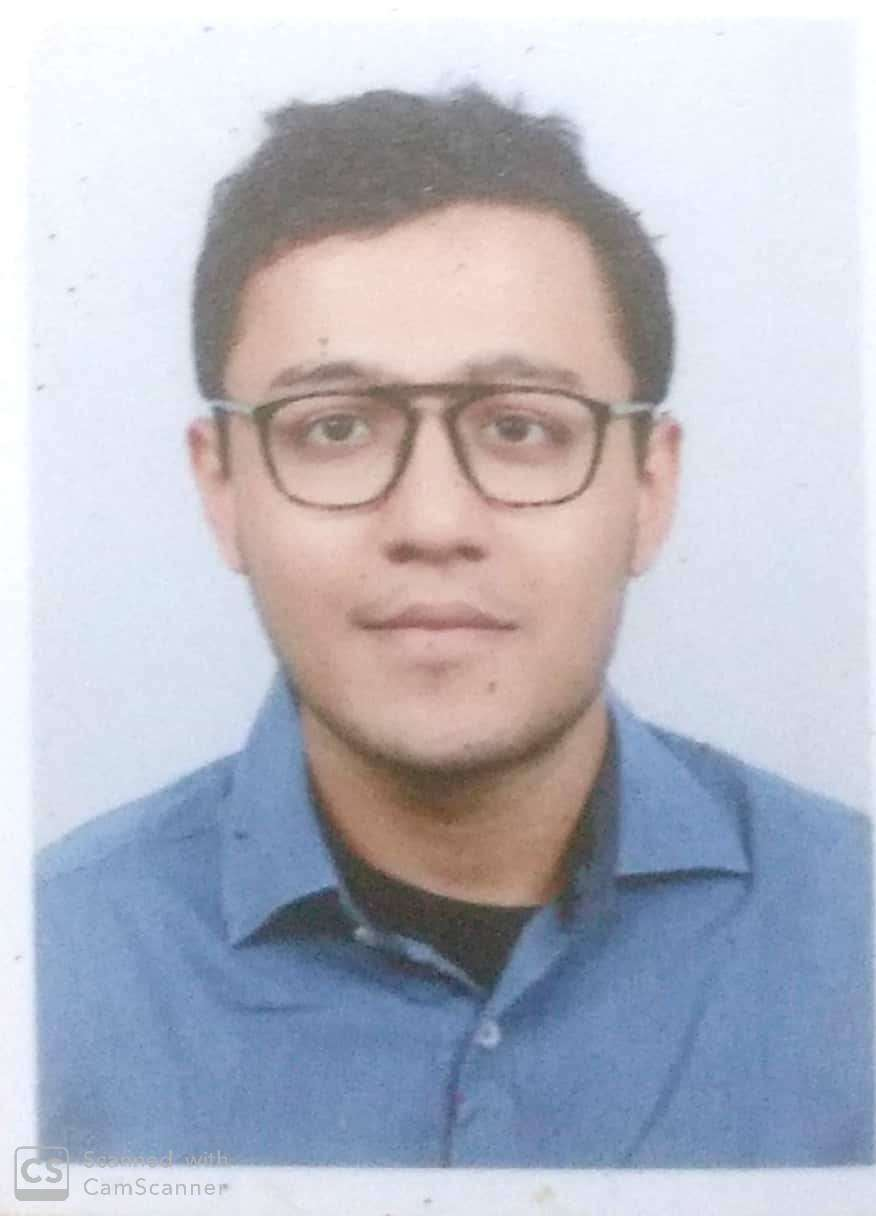
\includegraphics[width=2.5cm]{PHOTO.jpg}
\end{wrapfigure} 
%------------------------------------------
\textbf{}  \\
\textbf{{\Large Keval Mamaniya}}  \\
Email \hspace{0.2cm}  : keval.m@somaiya.edu \\
Contact : 9082491488 \\
Address : Flat no.9, Arun Niwas, Road No. 3, \\
\hspace{1.8cm}Chembur(E), Mumbai - 400071 \\ 
Linkedin : https://www.linkedin.com/in/kevalmamaniya
%\textbf{}  \\
%------------------------------------------------------------------------------%----------------------------Career Objective-------------------------------
\resheading{Career Objective}
\textbf{}  \\
Goal oriented engineer, with a zeal towards developing new solutions by applying knowledge of mechanical engineering in the field of robotics and keen enthusiast of learning new skills and concepts.\\
%-------------------Education--------------------------------------------------
\resheading{Education}

\begin{table}[h!]
	\begin{center}
		\begin{tabular}{|l|c|r|l|} % <-- Alignments: 1st column left, 2nd middle and 3rd right, with vertical lines in between
			\hline
			\hspace{0.2cm}\textbf{Year}\hspace{0.2cm} &\hspace{0.2cm} \textbf{Degree/Certificate}\hspace{0.2cm} &\hspace{0.2cm} \textbf{Institute}\hspace{2.5cm} &\hspace{0.2cm} \textbf{CGPA / Percent }\hspace{0.2cm}\\
			\hline
			\hspace{0.2cm}2013 & \hspace{0.2cm} Secondary School Certificate \hspace{0.2cm} & \hspace{0.2cm}Our Lady of Prepetual Succour High School\hspace{0.2cm} & \hspace{1.2cm} 88.00\% \hspace{0.2cm}\\
			\hspace{0.2cm}2015 & \hspace{0.2cm} Higher Secondary School Certificate \hspace{0.2cm} & \hspace{0.2cm}Our Lady of Prepetual Succour High School\hspace{0.2cm} & \hspace{1.2cm} 86.46\% \hspace{0.2cm}\\
			\hspace{0.2cm}2015 & \hspace{0.2cm} 1st Semester Btech  MECH \hspace{0.2cm} &\hspace{0.2cm}K.J. Somaiya College of Engineering\hspace{0.2cm} & \hspace{1.2cm} 6.35 \hspace{0.2cm}\\
			\hspace{0.2cm}2016 & \hspace{0.2cm} 2nd Semester Btech MECH \hspace{0.2cm} &\hspace{0.2cm}K.J. Somaiya College of Engineering\hspace{0.2cm} & \hspace{1.2cm} 7.42 \hspace{0.2cm}\\
			\hspace{0.2cm}2016 & \hspace{0.2cm} 3rd Semester Btech MECH \hspace{0.2cm} &\hspace{0.2cm}K.J. Somaiya College of Engineering\hspace{0.2cm} & \hspace{1.2cm} 7.38 \hspace{0.2cm}\\
			\hspace{0.2cm}2017 & \hspace{0.2cm} 4th Semester Btech MECH \hspace{0.2cm} &\hspace{0.2cm}K.J. Somaiya College of Engineering\hspace{0.2cm} & \hspace{1.2cm} 7.91 \hspace{0.2cm}\\
			\hspace{0.2cm}2017 & \hspace{0.2cm} 5th Semester Btech MECH \hspace{0.2cm} &\hspace{0.2cm}K.J. Somaiya College of Engineering\hspace{0.2cm} & \hspace{1.2cm} 8.32 \hspace{0.2cm}\\
			\hspace{0.2cm}2018 & \hspace{0.2cm} 6th Semester Btech MECH \hspace{0.2cm} &\hspace{0.2cm}K.J. Somaiya College of Engineering\hspace{0.2cm} & \hspace{1.2cm} 8.00 \hspace{0.2cm}\\
			\hspace{0.2cm}2018 & \hspace{0.2cm} 7th Semester Btech MECH \hspace{0.2cm} &\hspace{0.2cm}K.J. Somaiya College of Engineering\hspace{0.2cm} & \hspace{1.2cm} 8.96 \hspace{0.2cm}\\
			\hline
		\end{tabular}
	\end{center}
\end{table}

MECHANICAL \\
%--------------------------Projects----------------------------------------------------------------
\resheading{Projects}
\textbf{}  \\
\begin{enumerate}
	\item \textbf{Autonomous Surface Water Rover and Underwater Inspection System                                                                       } (July 2018 - Present): \\
	\begin{itemize}
		\item A system designed and developed for water quality monitoring of still water bodies and underwater infrastructure inspection along with data acquisition and visualization in real time.
		\item Designed and manufactured surface water rover with efficient propulsion system and compact underwater inspection system.
		\item System was successfully tested at Vashi mini seashore and various swimming pools.
	\end{itemize} 
	\item \textbf{MEDHA 2018} (July 2018): \\
	\textbf{Development of Palpatic tissue stiffness haptic device}\\
	\begin{itemize}
		\item Idea formulation, design and development of PoC for muscle stiffness measurement.
		\item Awarded with Certificate of Excellence for great teamwork, innovation and presentation.
	\end{itemize}
	\textbf{}  \\
	\textbf{}  \\
	\textbf{}  \\
	\textbf{}  \\
	\item \textbf{Team KJSCE Robocon} (August 2016 - May 2018)\\
	\begin{itemize}
		\item Member of the mechanical team for 2 years wherein I designed, fabricated \& tested mechanical systems like drive assembly, 2 DoF angle mechanism, suspension mechanism, pneumatic magnetic gripper and throwing mechanisms for different tasks to be completed in ABU Robocon.
		\item Senior mechanical head during 2nd year, I headed the mechanical team for designing and fabrication of Autonomous Robot.
		\item Managed marketing, administrative work and carrying out decisions along with senior team members.
		\item Secured 30th rank out of 107 teams in 2018 and 19th rank out of 113 teams in 2017 at Robocon Nationals, India.
	\end{itemize}
\end{enumerate}


\textbf{}  \\
\textbf{}  \\
\textbf{}  \\
%--------------------------------------Internship and Trainings---------------------------------
\resheading{Internships and Trainings}
\textbf{}  \\
\textbf{1. Mechanical Engineering Intern at  Machinecraft Thermoforming OEM (Dec 2018 - Feb 2019)} \\
\begin{itemize}
	\item Worked on a hydroponics project involving designing and manufacturing frame and Thermoforming trays for ebb flow system.
	\item Designed a material handling equipment to reduce cycle time of production for Thermoforming Machines.
	\item Worked with CAD/CAM team to understand basic functions of 3-axis CNC milling machine and to create 3D toolpath in Mastercam.
\end{itemize}
\textbf{}  \\
\textbf{}  \\
\textbf{2. Intern at Jeet Techno Solutions (June 2016 - July 2016)} \\
\begin{itemize}
	\item Designed various robotic parts and motors in Solidworks for documentation.
	\item Designed various modules to apprehend assembly movements in Solidworks.
\end{itemize}
\textbf{}  \\
\textbf{}  \\ 
%--------------------------------------Positions of Responsibilty---------------------------------
\resheading{Positions of Responsibilty}
\textbf{}  \\
\textbf{}   \\
\textbf{1. Senior Member Team KJSCE Robocon (May 2017- June 19 2018)} \\
\begin{itemize}
	\item Headed the junior members of mechanical team for developing different mechanisms.
	\item Team management and in-charge of all technical and non-technical decisions.
	\item Conducted robotics workshop at college for FE \& SE students to generate interest in the field of robotics.
	\item Played a role of controller at ABU Robocon 2018, India.
\end{itemize}
\textbf{}  \\
\textbf{}  \\
%--------------------------------------Technical Skills---------------------------------
\resheading{Technical Skills}
\textbf{}  \\


\begin{enumerate}
	\item Software Platforms Used:\\
	\begin{itemize}
		\item SolidWorks (Intermediate)
		\item AutoCAD (Intermediate)
		\item Ansys APDL \& Workbench  (Intermediate)
		\item Simscale (Basic)
		\item MATLAB (Basic)
		\item  MasterCAM (Basic)
	\end{itemize}
	
	\item Hands on Experience : 
	\begin{itemize}
		\item Lathe Machine
		\item CNC Router
		\item Laser Cutting Machine
		\item FDM 3D printer 
	\end{itemize}
\end{enumerate}
%--------------------------------------Soft Skills---------------------------------
\resheading{Soft Skills}
\textbf{}  \\

\begin{enumerate}
	\item Problem Solving
	\item Teamwork
	\item Ability to Work Under Pressure 
	\item Leadership
	\item Hardworking
	
	
\end{enumerate}
%--------------------------------------Extra Curricular Activities---------------------------------
\resheading{Extra-Curricular Activities}

\textbf{1. Social}  \\

\begin{itemize}
	\item Parvaah: Participated in “Hamara Station Hamari Shaan”, wherein task of beautification of suburban Railway Stations of                      
	Mumbai was undertaken.
	
	\item Arranged a voluntary blood donation camp on 21st June 2015, where a total of 82 voluntary donors donated blood. 
\end{itemize}
\textbf{2. Cultural}: Volunteered at Ghatkopar Carnival 2015, first cultural festival at a district level.

%--------------------------------------Co-Curricular Activities---------------------------------
\resheading{Co-Curricular Activities}
\textbf{}  \\
\begin{enumerate}
	\item Participated in e-YIC 2019 and won 'Best Hardware Award'in e-YIC Nationals.
	\item Participated in Prakalpa 2019 organized by ISTE and won 1st prize among final year Hardware projects in college.
	\item Participated in MEDHA 2018 organized by Betic, IIT Bombay and was awarded with Certificate of Excellence for great teamwork, innovation and presentation.
	\item Reached at Quarter Finals of IICDC contest organized by Texas Instruments in collaboration                                    
	with Department of Science and Technology. 
	
\end{enumerate}
%--------------------------------------Personal Details---------------------------------
\resheading{Personal Details}
\textbf{}  \\
Father's Name\hspace{0.05cm} : Vipul Mamaniya\\
Mother's name : Chetna Mamaniya\\
Date of Birth\hspace{0.26cm} : 1st August 1997\\
Nationality   \hspace{0.64cm}: Indian \\
Marital Status\hspace{0.20cm}: Single\\
%--------------------------------------References---------------------------------
\resheading{References}
\textbf{}  \\
\begin{enumerate}
	\item \textbf{Mr. Avinash A Prabhudesai} \\Mechanical Engineer\\avinashp@somaiya.edu\\
	\textbf{}  \\
	Prof. Avinash Prabhudesai was the project guide of my final year project "Autonomous Surface Water Rover \& Underwater Inspection System                                                                   ". His work in KJSCE includes a university grant project on a regenerative brake and a consultancy project on performance improvement of a sugarcane harvester. He was Faculty Advisor for KJSCE Robocon and has a US Patent for "Radiator Grille" which was granted in January 2017.
	\item \textbf{Mrs. Arati Phadke} \\ Associate Professor\\Electronics Dept.\\aratiphadke@somaiya.edu\\
	\textbf{}  \\ Prof. Arati Phadke was my eYIC mentor.She is also working as In charge of Accreditation for Institute since July 2014. She was the Head of Department of Electronics Engineering from May 2008 to June 2011 and Dean (Student’s Affairs ) from May 2005 to April 2008.
\end{enumerate}
%--------------------------------------Declaration---------------------------------
\resheading{Declaration}
\textbf{}\\
I, Keval Mamaniya declare that all the details in this document are true and a valid proof of the same will be made available if required.\\
\textbf{}  \\
\begin{tabular*}{7in}{l@{\extracolsep{\fill}}r}
	
	\textbf{{Date : }}  \textbf{\today} \\
\end{tabular*}
	\end{document}